\documentclass[10pt]{article}

\usepackage[margin=0.68in]{geometry}
\usepackage{amsmath,amssymb}
\usepackage{booktabs}
\usepackage{graphicx}
\graphicspath{{../figures/}}
\usepackage{array}
\usepackage{caption}
\usepackage{microtype}
\usepackage{enumitem}

\setlength{\parindent}{0pt}
\setlength{\parskip}{4pt}
\setlength{\textfloatsep}{7pt}
\setlength{\floatsep}{7pt}
\setlength{\intextsep}{7pt}
\captionsetup{font=small,skip=3pt}
\renewcommand{\arraystretch}{1.08}

\title{Instability and Damping in a One-Dimensional Gaussian Adjoint Sampler}
\author{}
\date{}

\begin{document}
\maketitle
\vspace{-1.4em}

\section{Problem and terminology}

We study a one-dimensional Gaussian-to-Gaussian problem with
\[
    p_{\mathrm{tar}} = N(1,0.02),
    \qquad
    p_0 = N(1.05,0.02),
    \qquad
    \sigma(t) \equiv 1,
    \qquad t\in[0,1].
\]
Here the \emph{drift} is the deterministic part of the sampling SDE. An \emph{outer iteration} means one cycle in which the current endpoint distribution is used to construct a new drift, after which the SDE is simulated again. In the learned cases, the drift is represented by a neural network. \emph{Reciprocal adjoint matching} refers to the Adjoint Sampling training rule that constructs regression targets from current terminal samples and the target density. A \emph{replay buffer} stores endpoint/gradient pairs from previous outer iterations and reuses them in later training. \emph{Damping} means replacing a newly trained network parameter vector by a convex combination of the previous and proposed parameter vectors.

Because the target and initial variances are matched, the exact Gaussian outer map predicts
\[
    m_{k+1}-1 = A\,(m_k-1),
    \qquad
    A = 1 + \frac{\log(0.02)}{1-0.02}
      \approx -2.99186.
\]
Thus the exact mean error alternates in sign and grows by a factor of about three per outer iteration. The continuous prediction for the mean is
\[
1.05,\quad 0.8504,\quad 1.4476,\quad -0.3390,\quad 5.0062.
\]
The numerical experiments use 500 time steps with the RMC \texttt{ql} time-grid option. Learned runs use three random seeds. Histograms for learned regimes pool the final samples across all three seeds; consequently, their pooled variance reflects both within-seed spread and variation in the terminal mean across seeds.

\begin{table}[h]
\centering
\small
\begin{tabular}{@{}p{0.21\linewidth}p{0.25\linewidth}p{0.26\linewidth}cc@{}}
\toprule
\textbf{Regime} & \textbf{Drift representation} & \textbf{How the drift is obtained} & \textbf{Replay} & \textbf{Damping} \\
\midrule
Affine oracle & Exact affine function & Closed-form Gaussian update from the current mean and variance & No & No \\
Learned affine & $3\times 64$ time-dependent neural network & Supervised regression onto the exact affine drift & No & No \\
Full Adjoint & Same neural network & Reciprocal adjoint matching from current terminal samples & 1000 & No \\
Full Adjoint + damping & Same neural network & Same as Full Adjoint & 1000 & $\eta=0.5$ \\
\bottomrule
\end{tabular}
\caption{The four regimes. In the damped case the first learned update is left undamped because $p_0$ is prescribed externally; parameter damping begins with the second outer update.}
\end{table}

\begin{table}[h]
\centering
\small
\begin{tabular}{@{}ll@{\qquad}ll@{}}
\toprule
\textbf{Quantity} & \textbf{Value} & \textbf{Quantity} & \textbf{Value} \\
\midrule
Training endpoints per outer step & 128 & Inner optimizer steps & 100 \\
Mini-batch size & 64 & Optimizer & Adam, $10^{-4}$ \\
Evaluation samples per seed & 10,000 & Oracle samples & 50,000 \\
Neural-network hidden widths & $64,64,64$ & Time steps & 500 \\
Terminal-gradient clip & 150 & Learned seeds & 0, 1, 2 \\
\bottomrule
\end{tabular}
\caption{Shared numerical settings for the learned experiments.}
\end{table}

\section{Affine oracle}

The oracle uses the exact affine Gaussian drift at every outer iteration, so it isolates the instability of the outer map from neural-network approximation and optimization error. The numerical mean trace is
\[
1.0500,\quad 0.8490,\quad 1.4371,\quad -0.3122,\quad 4.8179,
\]
which closely follows the continuous prediction. The variance remains near the target value: the final empirical variance is $0.02032$.

\begin{figure}[h]
\centering
\begin{minipage}[t]{0.49\linewidth}
\centering
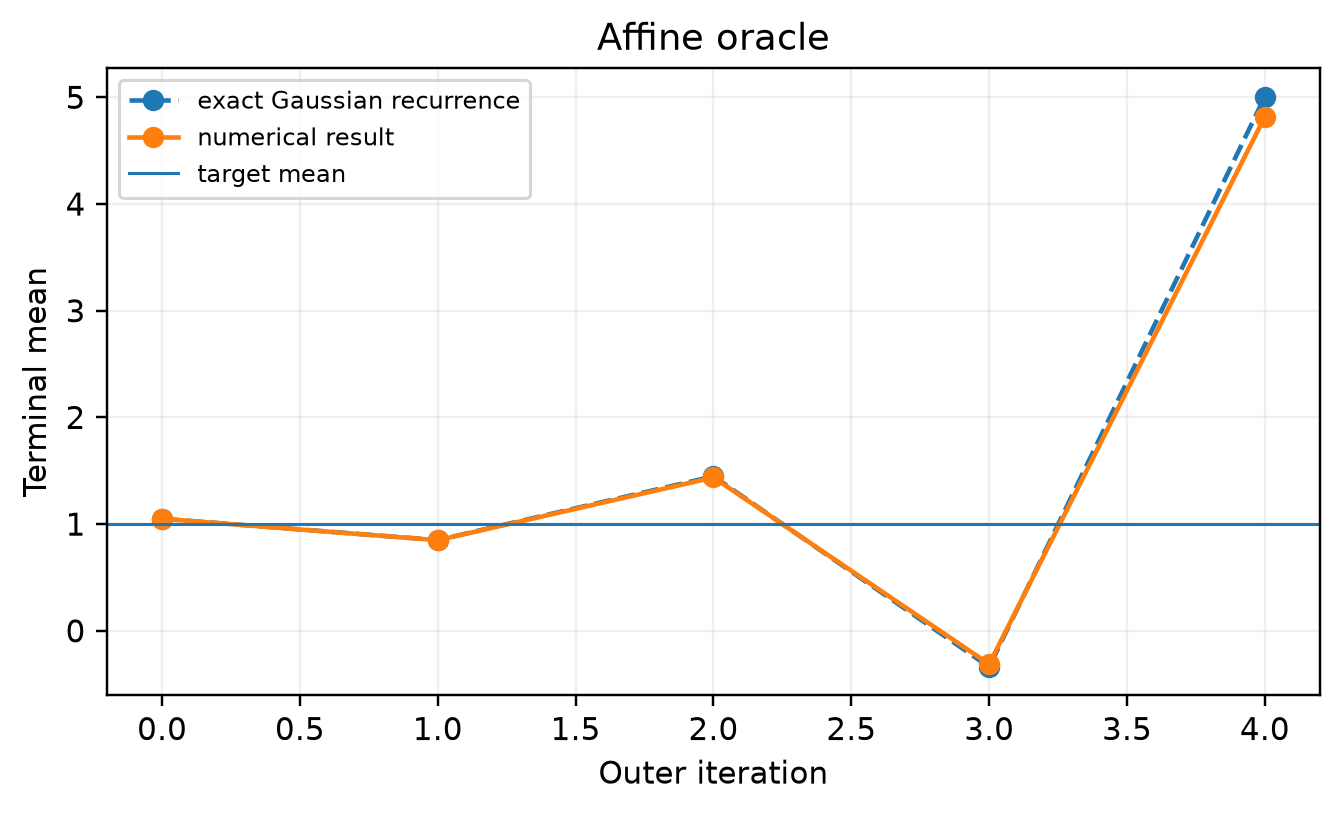
\includegraphics[width=\linewidth]{affine_oracle_mean.png}
\end{minipage}\hfill
\begin{minipage}[t]{0.49\linewidth}
\centering
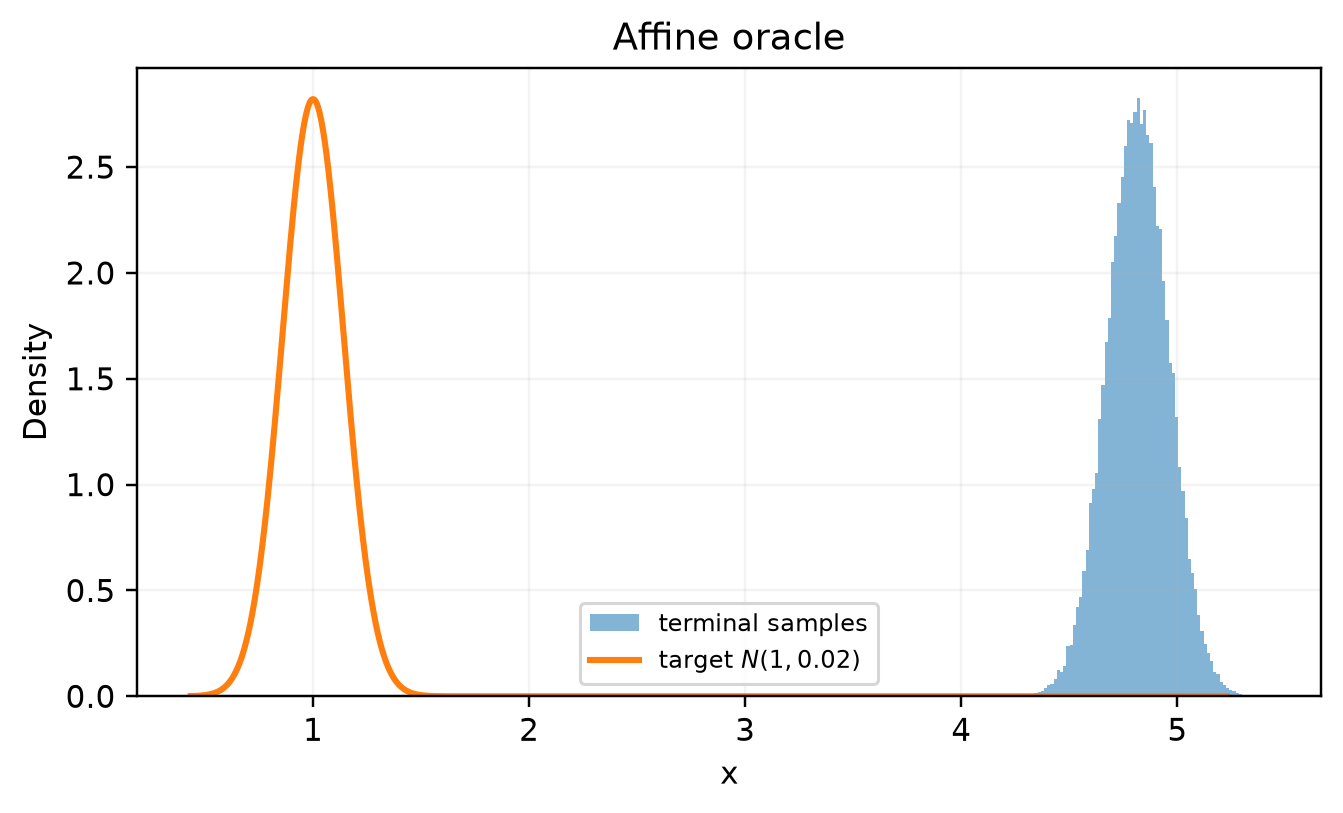
\includegraphics[width=\linewidth]{affine_oracle_hist.png}
\end{minipage}
\caption{Affine oracle. Left: terminal mean across outer iterations. Right: final terminal samples with the exact $N(1,0.02)$ density overlaid.}
\end{figure}

The oracle therefore gives the clean instability mechanism: the variance is essentially correct while the mean is driven away from the target by the alternating outer update.

\section{Learned affine drift}

This regime keeps the same neural-network architecture used by the practical sampler but trains it directly against the known affine drift. It removes the reciprocal-adjoint target construction and replay mechanism while retaining function approximation and finite optimization.

Averaged over the three seeds, the terminal mean follows
\[
1.0500,\quad -0.3775,\quad 0.5597,\quad 2.5374,\quad 0.4758.
\]
The final seed-to-seed standard deviation of the mean is $0.1263$. The pooled final variance is $0.2069$, more than ten times the target variance.

\begin{figure}[h]
\centering
\begin{minipage}[t]{0.49\linewidth}
\centering
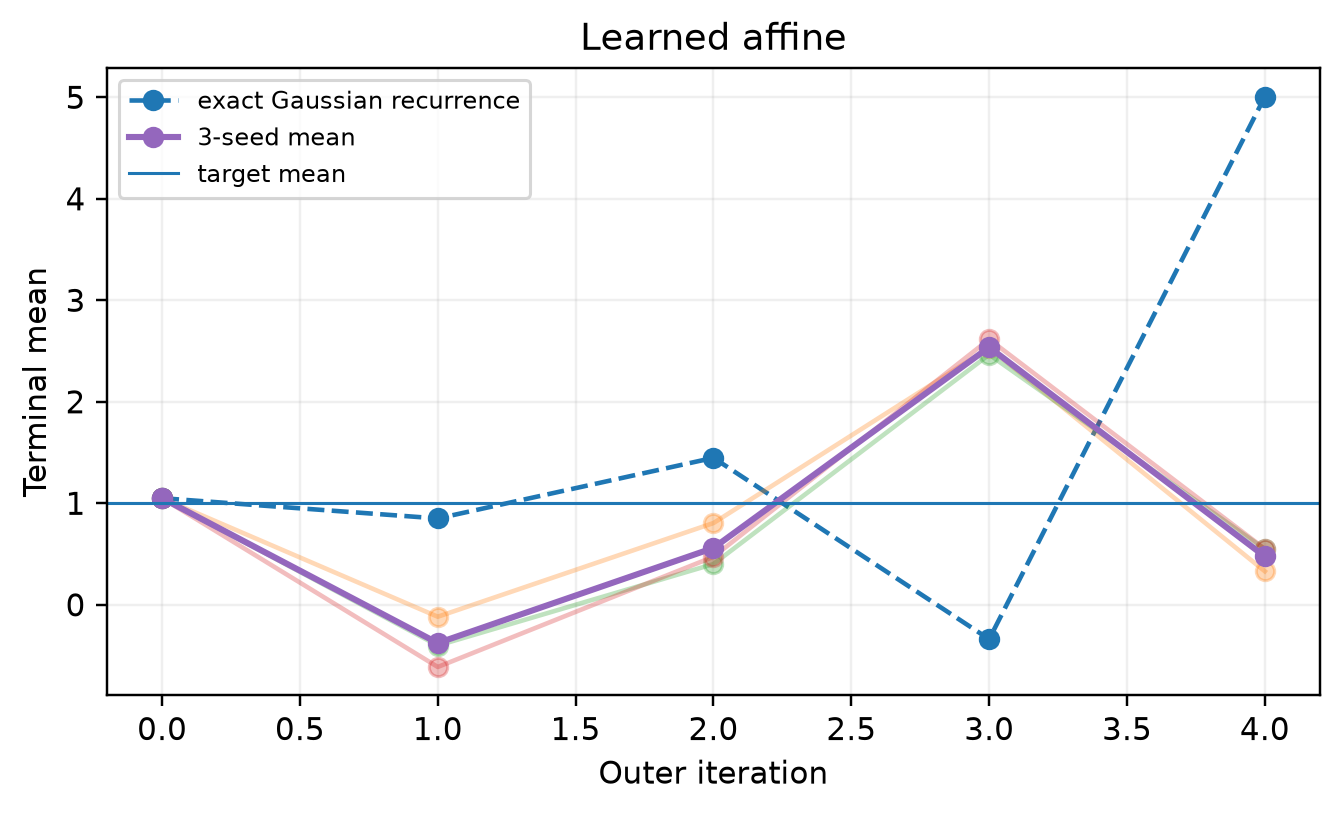
\includegraphics[width=\linewidth]{learned_affine_mean.png}
\end{minipage}\hfill
\begin{minipage}[t]{0.49\linewidth}
\centering
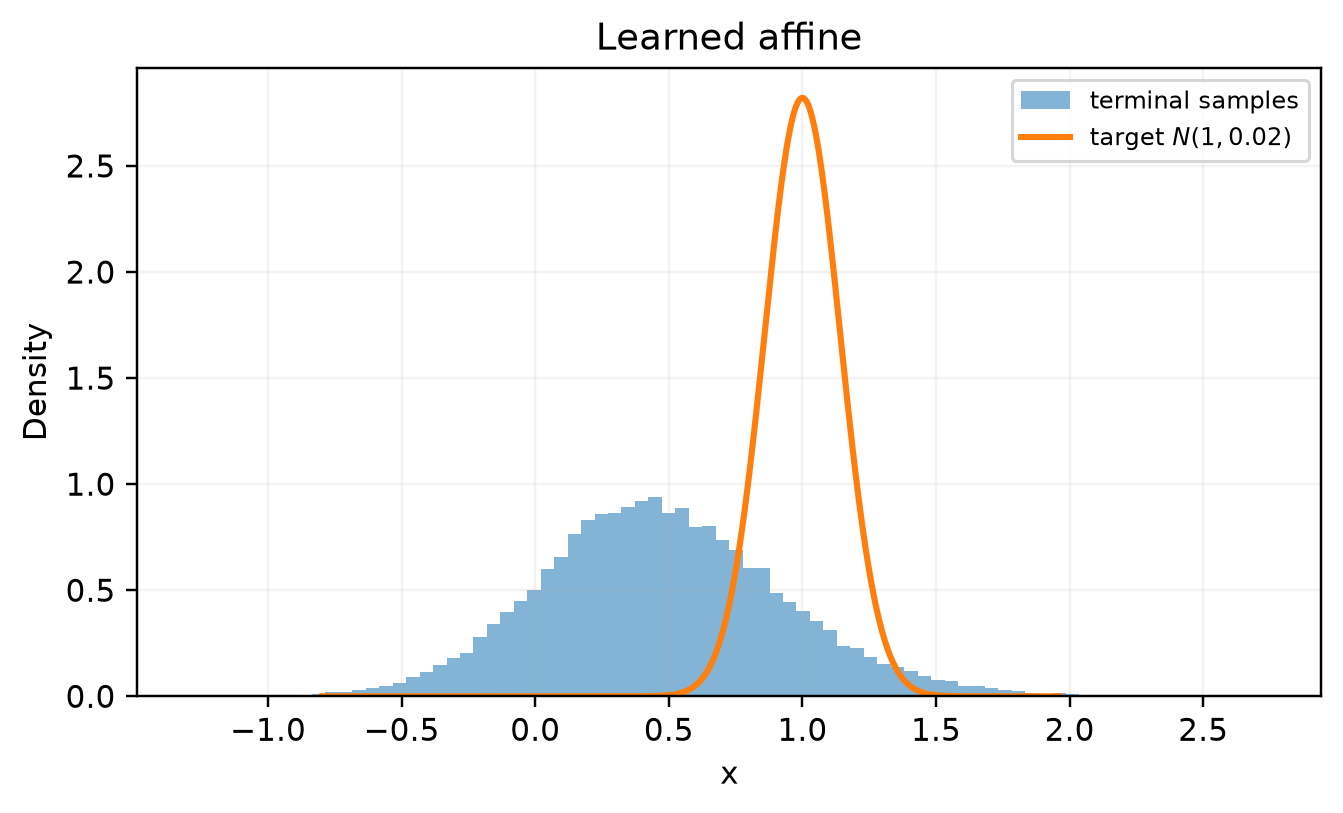
\includegraphics[width=\linewidth]{learned_affine_hist.png}
\end{minipage}
\caption{Learned affine drift. Thin curves show individual seeds and the heavier curve shows their mean. The histogram pools the final samples from all three seeds.}
\end{figure}

The mean remains strongly oscillatory, but the learned dynamics no longer follow the exact Gaussian recurrence. The variance inflation shows that fitting the drift with a finite neural network changes both the mean and contraction properties of the update.

\section{Full Adjoint sampler}

The full sampler uses reciprocal adjoint matching, rollout feedback, a 1000-sample replay buffer, and terminal-gradient clipping at 150. The mean averaged across seeds is
\[
1.0500,\quad -0.3005,\quad 1.0064,\quad 2.1552,\quad 1.5859.
\]
The final seed-to-seed standard deviation of the mean is $1.5032$, substantially larger than in the learned-affine experiment. The three final means are $0.8464$, $0.5957$, and $3.3156$. The pooled terminal variance is $1.6604$.

\begin{figure}[h]
\centering
\begin{minipage}[t]{0.49\linewidth}
\centering
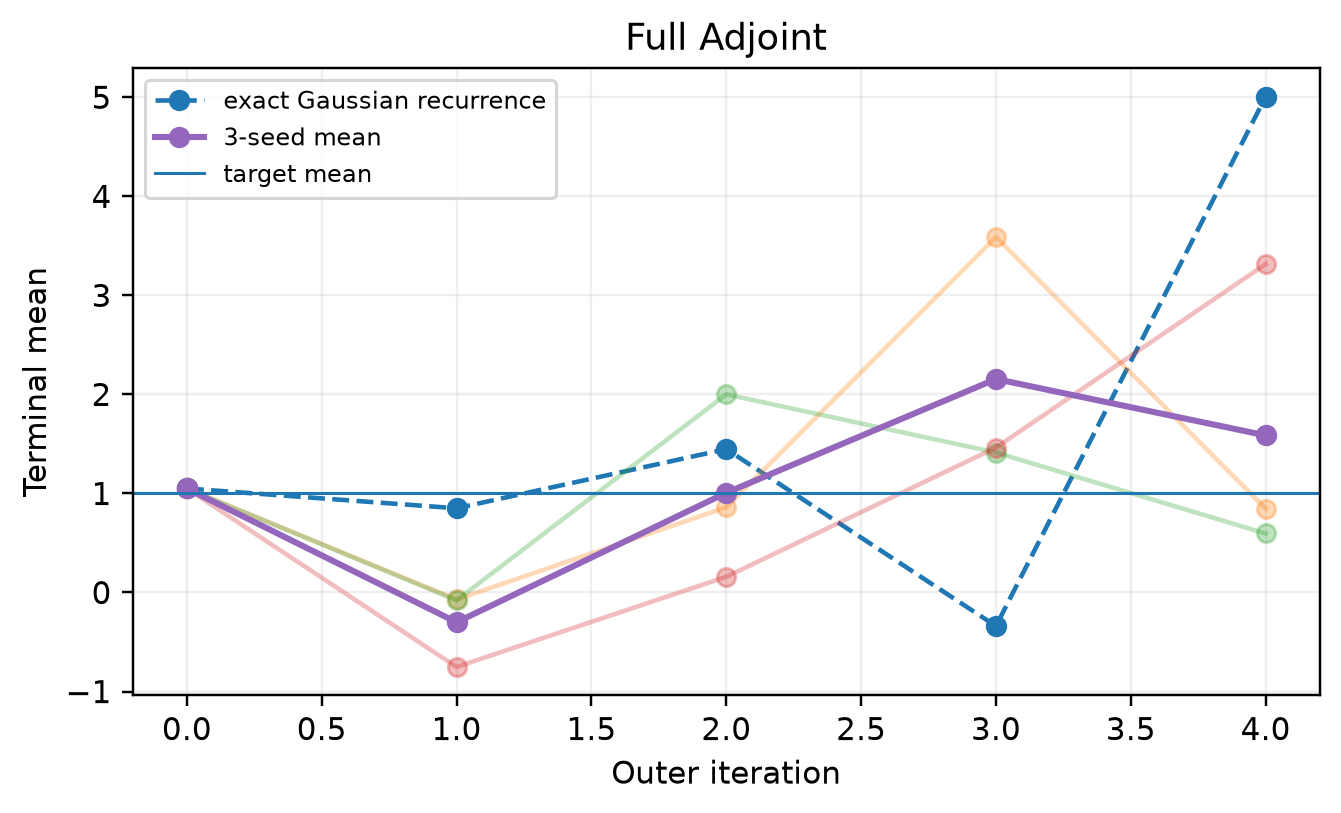
\includegraphics[width=\linewidth]{full_adjoint_mean.png}
\end{minipage}\hfill
\begin{minipage}[t]{0.49\linewidth}
\centering
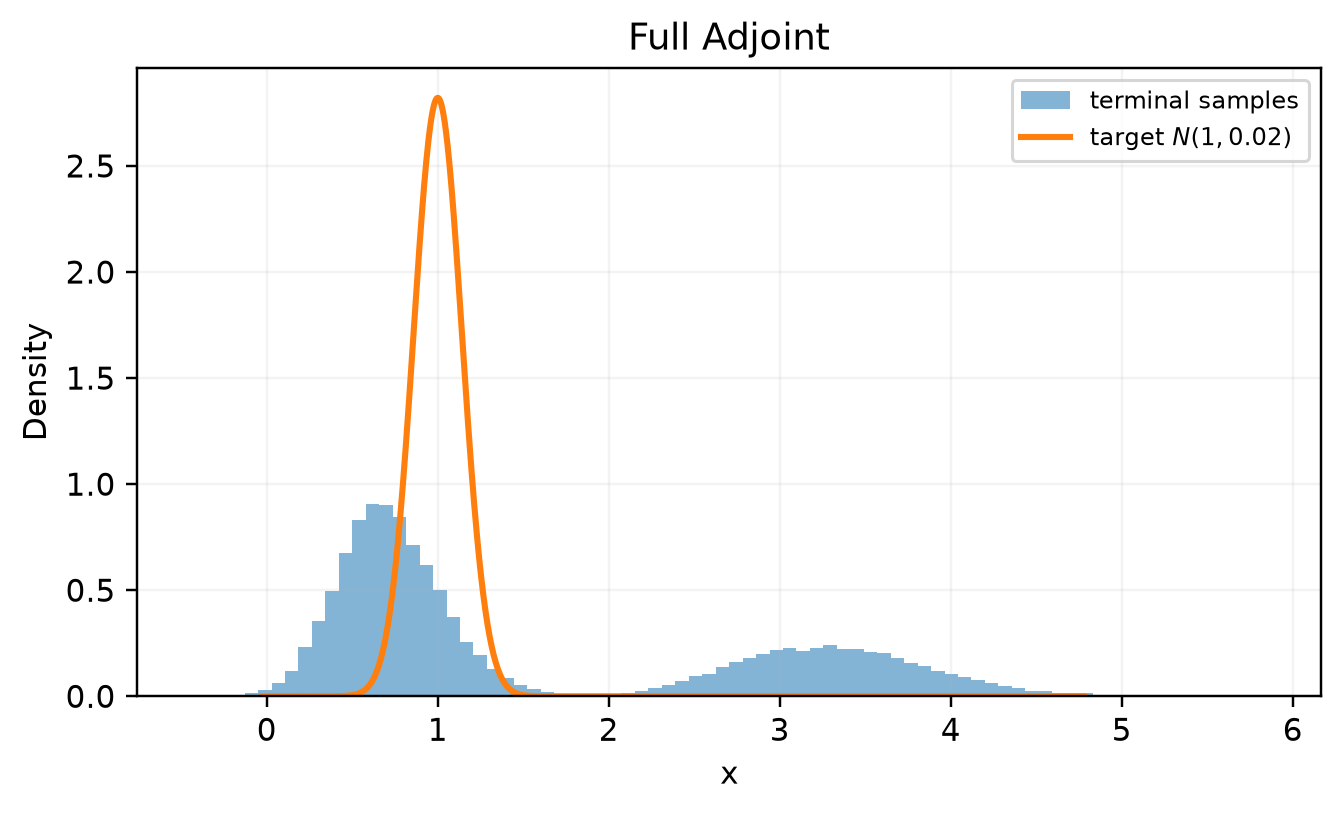
\includegraphics[width=\linewidth]{full_adjoint_hist.png}
\end{minipage}
\caption{Full Adjoint sampler. The terminal distribution is broad and strongly seed-dependent after four outer iterations.}
\end{figure}

The practical training machinery substantially changes the exact outer-map dynamics. Instability remains visible through oscillation and seed sensitivity, but the dominant failure is now a combination of mean error and severe variance inflation. Terminal-gradient clipping is active in a few outer iterations, so the run also enters the safeguard regime of the implementation.

\section{Full Adjoint sampler with damping}

The damped sampler is identical to the full sampler except that, after each inner training block from the second outer iteration onward, the proposed neural-network parameters $\widehat\theta_{k+1}$ are replaced by
\[
    \theta_{k+1}
    = (1-\eta)\theta_k + \eta\widehat\theta_{k+1},
    \qquad \eta=0.5.
\]
The first update is intentionally undamped, so the first-step results agree exactly with the undamped sampler. If the same relaxation acted directly on the scalar mean error, the ideal multiplier would be
\[
    1-\eta+\eta A \approx -0.99593,
\]
which is only barely contractive. Parameter averaging in a nonlinear network is not identical to scalar mean relaxation, so this value serves only as a reference.

The three-seed mean trace is
\[
1.0500,\quad -0.3005,\quad 0.1383,\quad 0.8518,\quad 1.6319.
\]
The final seed-to-seed standard deviation of the mean falls from $1.5032$ without damping to $0.8402$ with damping. The pooled terminal variance falls from $1.6604$ to $0.8487$, although it remains far above the target variance $0.02$.

\begin{figure}[h]
\centering
\begin{minipage}[t]{0.49\linewidth}
\centering
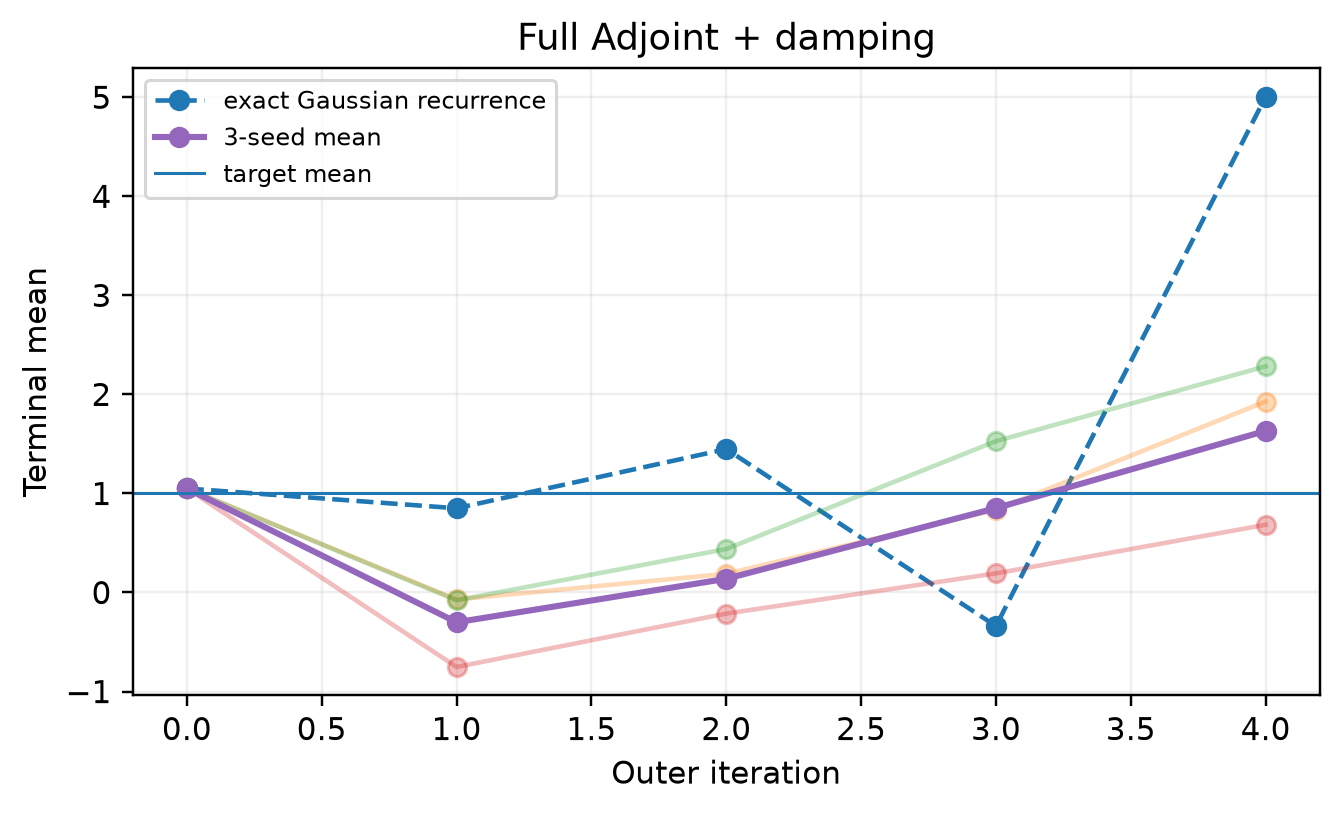
\includegraphics[width=\linewidth]{full_adjoint_damped_mean.png}
\end{minipage}\hfill
\begin{minipage}[t]{0.49\linewidth}
\centering
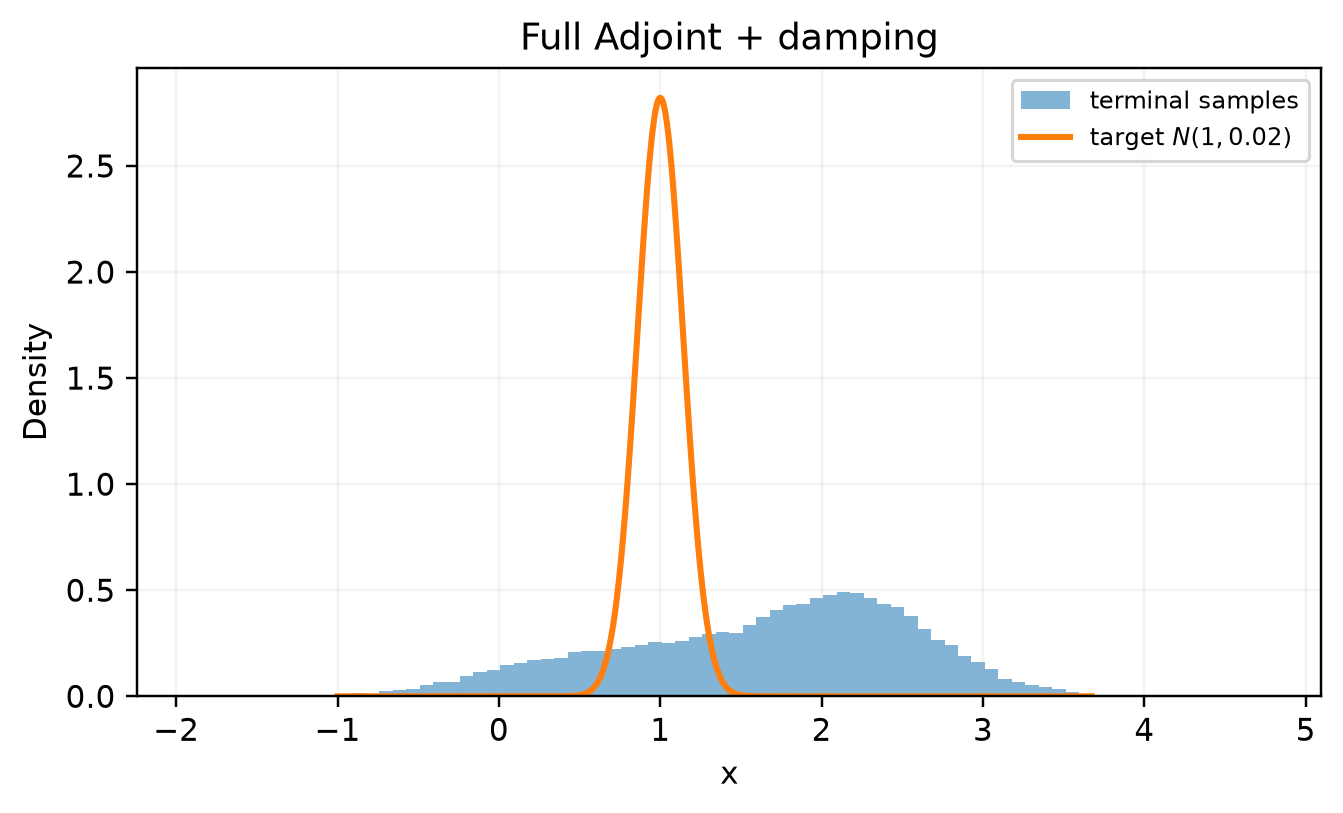
\includegraphics[width=\linewidth]{full_adjoint_damped_hist.png}
\end{minipage}
\caption{Full Adjoint sampler with parameter damping $\eta=0.5$. The dashed curve in the mean panel is the undamped exact Gaussian recurrence and is shown only as a reference. Damping reduces seed-to-seed spread and terminal variance but does not recover the target distribution within four outer iterations.}
\end{figure}

\section{Comparison}

\begin{table}[h]
\centering
\small
\begin{tabular}{@{}lrrr@{}}
\toprule
\textbf{Regime} & \textbf{Final pooled mean} & \textbf{Final pooled variance} & \textbf{SD of final seed means} \\
\midrule
Affine oracle & 4.8173 & 0.0203 & -- \\
Learned affine & 0.4758 & 0.2069 & 0.1263 \\
Full Adjoint & 1.5859 & 1.6604 & 1.5032 \\
Full Adjoint + damping & 1.6319 & 0.8487 & 0.8402 \\
\bottomrule
\end{tabular}
\caption{Terminal comparison after four outer iterations. The learned pooled statistics combine all three seeds.}
\end{table}

The experiment separates three effects. First, the exact Gaussian update has a genuine outer-iteration instability even while preserving the target variance accurately. Second, finite neural-network fitting substantially modifies that ideal map and introduces variance error. Third, the full reciprocal-adjoint/replay implementation is considerably more seed-sensitive than the direct affine regression experiment. Parameter damping reduces that seed sensitivity and cuts the pooled terminal variance by roughly one half, but $\eta=0.5$ is near the scalar stability boundary for this target variance and does not yield convergence over the four iterations tested. These results support damping as a stabilizing modification while also showing that the practical sampler has approximation and variance-control errors beyond the one-dimensional mean instability predicted by the Gaussian analysis.

\end{document}
